\documentclass[runningheads,envcountsame,orivec]{llncs}
\usepackage[T1]{fontenc}
\usepackage[utf8]{inputenc}
\usepackage{lmodern}
\usepackage{microtype}
\usepackage{amsmath,amssymb,mathtools}
\usepackage{booktabs}
\usepackage{tikz}
\usepackage[hidelinks]{hyperref}
\urlstyle{same}

\newcommand{\E}{\mathbb E}
\newcommand{\PP}{\mathbb P}
\newcommand{\ind}{\mathbf 1}
\newcommand{\ch}{\operatorname{ch}}
\newcommand{\parnt}{\operatorname{par}}
\newcommand{\nil}{\bot}
\newcommand{\R}{\mathcal R}
\newcommand{\coef}[2]{[z^{#1}]#2}


\begin{document}
\title{Exact Matching under Affine Preferential Attachment: Update Laws, Gaussian Fluctuations, and Extremes}
\titlerunning{Matching under Affine Preferential Attachment}
\author{Marek Ga\l{}\k{a}zka}
\authorrunning{M. Ga\l{}\k{a}zka}
\institute{Faculty of Mathematics and Computer Science,\\
Adam Mickiewicz University, Pozna\'n, Poland}
\maketitle

\begin{abstract}
Pairing as many adjacent vertices as possible in a growing tree requires
repeated corrections to a matching. How much work do these corrections
take, and how large can a single update become? We answer these questions
for the standard local algorithm under affine preferential attachment:
a new leaf selects parent $v$ with weight $1+\beta|\ch(v)|$, where
$\ch(v)$ is its set of children and $\beta>0$ is fixed.
We prove a nondegenerate central limit theorem for cumulative
vertex inspections, with linear asymptotic variance and an explicit
constant correction to the linear mean. The largest update lies almost
surely within a bounded additive distance of an explicit Lambert-$W$
centering. We also give constant expected update and recourse bounds,
an integral formula for the limiting update law, and sharp factorial
tail asymptotics. The proofs combine weighted sensitivity generating
functions, an approximation preserving the mean at every fringe size,
and local resampling with an unchanged exterior state history.
All results transfer to attachment proportional to degree plus a fixed
offset; ordinary degree attachment has expected inspection count at
most $3/2$. The algorithm is known; the contribution is its stochastic
cost analysis under reinforcement.
\keywords{Preferential attachment \and Dynamic matching \and Central limit theorem \and Extreme updates \and Fringe subtrees}
\end{abstract}

\section{Introduction}

A matching pairs adjacent vertices so that no vertex belongs to two
pairs. Suppose a tree grows one leaf at a time and we want as many
pairs as possible after every insertion. One new vertex can trigger a
chain of corrections, although the optimum number of pairs increases
by at most one; Figure~\ref{fig:intro-update} shows a small example.
How much work do these corrections require over the
lifetime of the tree, and how large can a single update become?
A bounded expected update cost gives an average budget, but leaves
its fluctuations and the largest delay unresolved.

\begin{figure}[t]
\centering
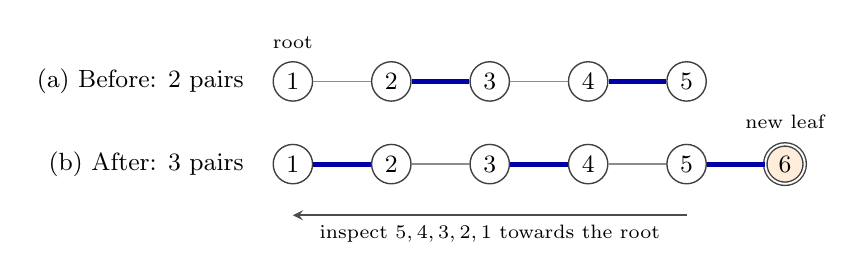
\begin{tikzpicture}[
 x=1cm,y=1cm,
 vertex/.style={circle,draw=black!75,fill=white,line width=.5pt,
                minimum size=5mm,inner sep=0pt,font=\small},
 tree edge/.style={draw=black!45,line width=.5pt},
 matched/.style={draw=blue!65!black,line width=1.8pt},
 every node/.style={font=\small}]
 \node[anchor=east] at (-.5,0) {(a) Before: 2 pairs};
 \node[anchor=east] at (-.5,-1.05) {(b) After: 3 pairs};
 \foreach \i/\x in {1/0,2/1.25,3/2.5,4/3.75,5/5} {
   \node[vertex] (a\i) at (\x,0) {\i};
   \node[vertex] (b\i) at (\x,-1.05) {\i};
 }
 \node[vertex,double,double distance=.7pt,fill=orange!15]
   (b6) at (6.25,-1.05) {6};
 \foreach \u/\v in {1/2,2/3,3/4,4/5}
   \draw[tree edge] (a\u)--(a\v);
 \foreach \u/\v in {1/2,2/3,3/4,4/5,5/6}
   \draw[tree edge] (b\u)--(b\v);
 \foreach \u/\v in {2/3,4/5}
   \draw[matched] (a\u)--(a\v);
 \foreach \u/\v in {1/2,3/4,5/6}
   \draw[matched] (b\u)--(b\v);
 \node[anchor=south,font=\scriptsize] at (0,.29) {root};
 \node[anchor=south,font=\scriptsize] at (6.25,-.72) {new leaf};
 \draw[->,>=stealth,draw=black!70,line width=.6pt]
   (5,-1.70)--node[below,font=\scriptsize]
   {inspect $5,4,3,2,1$ towards the root} (0,-1.70);
\end{tikzpicture}
\caption{An update chain in the standard local algorithm. Vertex 1 is
the root; thick blue edges form the maintained maximum matching.
Inserting leaf 6 makes the algorithm inspect all five old vertices:
two matched edges are removed and three are added. The optimum
matching size increases only from two to three.}
\label{fig:intro-update}
\end{figure}

We study affine preferential attachment: vertices with more children
are more likely to receive the next leaf. A vertex with $c$ children
has selection weight $1+\beta c$, where $\beta>0$ is fixed.
The standard local matching algorithm revises information from the
insertion point towards the root and stops when no further change is
needed. Successive update costs are dependent because they act on the
same evolving tree.

\paragraph{Contribution.}
Our contribution is a probabilistic analysis of this execution history.
The algorithm and its matching recurrence are classical.
For a tree grown to $N$ vertices, we establish three levels of control:
\begin{itemize}
\item A single update has bounded expected cost and a limiting law with
sharp factorial tails; the expected number of changed matching edges
is also bounded.
\item Total vertex inspections have a linear mean, an explicit constant
mean correction, and Gaussian fluctuations of order $\sqrt N$, with
a strictly positive limiting variance coefficient.
\item The largest update grows as $\log N/\log\log N$. More precisely,
it eventually stays almost surely within a bounded distance of an
explicit centering, giving a second-order asymptotic expansion.
\end{itemize}
Thus the results describe both typical cumulative work and rare large
updates of exact matching maintenance under reinforcement.

\paragraph{Related work.}
Acar et al.~\cite{AcarEtAl2004} develop a general framework for
propagating input changes through computations, with applications to
dynamic trees. For exact matching cardinality, Gupta and
Sharma~\cite{GuptaSharma2009} give an $O(\log n)$ worst-case update
algorithm on arbitrary dynamic trees. In the incremental model,
Tirodkar and Vishwanathan~\cite{TirodkarVishwanathan2019} obtain
constant worst-case update time with a randomized $3/2$-approximation
in expectation on trees. Our guarantees concern an exact local
algorithm under a specified random insertion law; they do not improve
these bounds for arbitrary update sequences.

The affine model belongs to the increasing-tree growth families
characterized by Panholzer and Prodinger~\cite{PanholzerProdinger2007}.
Rudas, T\'oth and Valk\'o~\cite{RudasTothValko2007} place preferential
tree growth in a general branching-process framework. Janson
\cite{Janson2020} studies independence numbers, and hence matching
sizes, in random trees including preferential trees; his recurrence
also supplies the static basis for our algorithm. The parameter here
records the work across all insertion times, not only the optimum in
the final tree.

\paragraph{Why additional analysis is needed.}
The increasing-tree fringe estimates of Seelbach Benkner and Wagner
\cite{SeelbachWagner2022} and the additive-functional central limit
theorem of Ralaivaosaona and Wagner~\cite{RalaivaosaonaWagner2019}
are inputs. Applying the latter requires control of an unbounded
history score. We prove a variance estimate after centering at each
subtree size, and a local resampling argument establishes positive
limiting variance. For the maximum, we control counts of small
subtrees that certify a large update, addressing dependence between
insertion times. These arguments use fixed positive reinforcement;
we do not claim estimates uniform as $\beta$ tends to zero.

\section{Model, algorithm, and results}\label{sec:model}

Start with one root and fix $\beta>0$. Conditional on $T_n$, vertex
$n+1$ chooses parent $v$ with probability
\begin{equation}\label{eq:affineparent}
 \frac{1+\beta|\ch(v)|}{Z_n},\qquad Z_n=(1+\beta)n-\beta.
\end{equation}
Here $\ch(v)$ is the set of children; at the root this convention
differs from ordinary degree attachment. Vertices retain their arrival
labels. The parent is supplied to the algorithm, so sampling it is
outside the measured cost. There are no deletions or edge weights.

For a rooted tree $T$, let $T_v$ be the fringe subtree consisting of
$v$ and all its descendants. Define
\begin{equation}\label{eq:state}
 d(v)=\ind\{\text{some }u\in\ch(v)\text{ has }d(u)=0\}.
\end{equation}
Leaves have state zero. After adding a leaf, recompute its parent's
state, then ascend while states change. Stop at the first unchanged
state or after processing the root. Let $K_n$ count changed old
vertices, $U_n$ inspected old vertices, and $R_n$ the indicator that
the root changes. Thus $U_n=K_n+1-R_n$. Put
\[
 S_N=\sum_{n=1}^{N-1}U_n,\qquad
 W_N=\max_{1\le n<N}U_n,\qquad S_1=W_1=0.
\]

\begin{lemma}\label{lem:implementation}
For every leaf-insertion history, choosing one zero-state child $c(v)$
at each one-state vertex gives a maximum matching
$M=\{\{v,c(v)\}:d(v)=1\}$, of size $\sum_vd(v)$.
This matching can be maintained in $O(1+U_n)$ time per insertion,
with at most $K_n+2$ edge changes, linear space, and constant-time
cardinality, mate, and edge-membership queries between updates.
\end{lemma}
\begin{proof}
If $\nu_0(T_v)$ is the optimum leaving $v$ unmatched within its
fringe, then $\nu_0(T_v)=\sum_u\nu(T_u)$.
The difference $\nu(T_v)-\nu_0(T_v)$ is zero or one and obeys
\eqref{eq:state}, by considering a match from $v$ to a child.
The selected edges are disjoint because their parent endpoints have
state one and their child endpoints have state zero.

Maintain each vertex's state, parent, a doubly linked list of its
zero-state children, and its selected child. Retain a valid selection,
otherwise take the list head. Each upward inspection and propagation
of a changed child into its parent's list takes constant time.
A changed state adds or removes one selected edge; the final unchanged
vertex may replace one edge by another. Delete all obsolete edges
before adding replacements. A global counter and mate pointers give
the query bounds. The word-RAM stores identifiers and counters in
single words.
\end{proof}

\paragraph{Analytic notation.}
Write $\zeta=(1+\beta)^{-1}$, $\theta=1-\zeta$, and
$\phi(x)=(1-\beta x)^{-1/\beta}$. The weighted tree EGF is
\[
 \mathcal T(z)=\frac{1-(1-z/\zeta)^{\beta/(1+\beta)}}\beta.
\]
The state-restricted EGFs $A_0,A_1$ are determined by
$A_0'=\phi(A_1)$, $A_0+A_1=\mathcal T$, $A_0(0)=A_1(0)=0$.
Define
\begin{equation}\label{eq:affinelimitfunctions}
 \begin{gathered}
 H(z)=\int_0^z\phi'(A_1(t))\,dt,\qquad
 H_\beta=H(\zeta),\quad h_\beta=H'(\zeta),\\
 \Phi_\beta(s)=\zeta\int_0^1(1-x)^{\zeta-1}
       \frac{e^{sH(\zeta x)}-1}{s}\,dx,\qquad
 \mu_\beta=1+\Phi_\beta(1).
 \end{gathered}
\end{equation}
At $s=0$ the quotient means $H(\zeta x)$.
Both $H_\beta$ and $h_\beta$ are finite and positive, as proved below.

\begin{theorem}\label{thm:affine}
For every $n\ge1$,
\begin{equation}\label{eq:affinemeans}
 \E K_n\le\frac n{Z_n},\qquad
 \E U_n\le1+\frac{n-1}{Z_n},\qquad
 \E|M_{n+1}\triangle M_n|\le2+\frac n{Z_n}\le3.
\end{equation}
Hence expected update time is constant and expected total time is
linear. Uniformly in $n,k\ge1$,
\begin{equation}\label{eq:factorialupper}
 \PP(K_n\ge k)\le h_\beta\frac{H_\beta^{k-1}}{(k-1)!}.
\end{equation}
\end{theorem}
These expectations average over the entire growth history, not over
the next insertion conditional on every possible realized tree.

\begin{theorem}\label{thm:affinelimit}
There is a nonnegative integer-valued $K_\beta$ such that
$K_n\xrightarrow{d}K_\beta$ and $U_n\xrightarrow{d}K_\beta+1$.
For $s\ge0$ and integers $k\ge1$,
\begin{align}
 \E s^{K_\beta}&=1+(s-1)\Phi_\beta(s),\label{eq:affinelimitpgf}\\
 \PP(K_\beta\ge k)&=\frac{\zeta}{k!}\int_0^1
 (1-x)^{\zeta-1}H(\zeta x)^k\,dx.\label{eq:affinelimittails}
\end{align}
Every fixed polynomial moment converges, as does $\E s^{K_n}$ for
each fixed $s>0$. In particular $\E U_n\to\mu_\beta\le1+\zeta$.
Furthermore,
\begin{equation}\label{eq:affinelimitsharp}
 \PP(K_\beta\ge k)\sim
 \Gamma(1+\zeta)\left(\frac{H_\beta}{\zeta h_\beta}\right)^\zeta
 \frac{H_\beta^k}{k!\,k^\zeta}.
\end{equation}
\end{theorem}

\begin{theorem}\label{thm:affinerefinedmax}
Define
\begin{equation}\label{eq:lambertcenter}
 r_\beta(N)=\frac{\log N}
 {\operatorname W_0(\log N/(eH_\beta))},\qquad
 \operatorname W_0(x)e^{\operatorname W_0(x)}=x.
\end{equation}
Then
\begin{equation}\label{eq:boundedmaximum}
 W_N=r_\beta(N)+O_\beta(1)\qquad\text{almost surely}.
\end{equation}
Writing $L=\log N$, $\ell=\log\log N$, $m=\log\log\log N$,
\begin{equation}\label{eq:secondordermaximum}
 W_N=\frac L\ell+
 \frac{L(m+1+\log H_\beta)}{\ell^2}
 +O_\beta\!\left(\frac{Lm^2}{\ell^3}\right)
 \quad\text{almost surely}.
\end{equation}
\end{theorem}
The bounded window has a deterministic width after an almost surely
finite random threshold. No Gumbel limit is asserted.

\begin{theorem}\label{thm:affinetotal}
There is an explicit finite $c_\beta$, given in
\eqref{eq:meancorrection}, such that
\begin{equation}\label{eq:affinetotal}
 \E S_N=\mu_\beta N-c_\beta+o(1).
\end{equation}
\end{theorem}

\begin{theorem}\label{thm:affineCLT}
There is a constant $0<\sigma_\beta^2<\infty$ such that
\begin{equation}\label{eq:fullPAclt}
 \frac{S_N-\mu_\beta N}{\sigma_\beta\sqrt N}
 \xrightarrow{d}\mathcal N(0,1),\qquad
 \operatorname{Var}(S_N)=\sigma_\beta^2N+o(N).
\end{equation}
In particular,
\begin{equation}\label{eq:CLTabsmean}
 \sqrt N\,\E|S_N/N-\mu_\beta|
 \longrightarrow\sigma_\beta\sqrt{2/\pi}.
\end{equation}
\end{theorem}
Thus the mean absolute error has the exact order $N^{-1/2}$.
The proof gives a positive lower bound on $\sigma_\beta^2$ and a
convergent approximation to it, without a closed-form evaluation.

\begin{corollary}\label{cor:degree}
Start from one edge, root it at either endpoint, and attach each new
leaf proportionally to $\deg(v)+\delta$, where $\delta>-1$ is fixed.
Count creation of the seed edge as $U_1=1$.
For $n\ge2$,
\begin{equation}\label{eq:degreemean}
 \E U_n\le1+\frac{(1+\delta)(n-1)}{(2+\delta)n-2}.
\end{equation}
In particular $\E U_n\le3/2$ for ordinary degree attachment.
Update time and recourse have constant expectation. With
$\beta=1/(1+\delta)$, Theorems~\ref{thm:affinelimit},
\ref{thm:affinerefinedmax}, and~\ref{thm:affineCLT} hold with the same
limit variables and constants. The mean is $\mu_\beta N+O_\beta(1)$.
\end{corollary}

\section{Sensitivity and fringe structure}\label{sec:sensitivity}

Give an increasing tree weight
$w_\beta(T)=\prod_v\prod_{j=0}^{|\ch(v)|-1}(1+\beta j)$ and put
$\tau_k=\prod_{i<k}Z_i$. Its probability is $w_\beta(T)/\tau_k$.
Let $B_\beta(T)$ sum insertion weights over sites that change the
root state. Let $m$ be the number of zero-state children; when $m=1$,
denote its unique zero-state child by $u_0$. Then
\begin{equation}\label{eq:Brec}
 B_\beta(T)=
 \begin{cases}
 1+\beta|\ch(r)|+\sum_{u\in\ch(r)}B_\beta(T_u),&m=0,\\
 B_\beta(T_{u_0}),&m=1,\\
 0,&m\ge2.
 \end{cases}
\end{equation}
Indeed, a child affects its parent exactly when all other children
have state one. Let $C(z)$ be the weighted EGF with additional
factor $B_\beta(T)$. This recurrence yields
$C'=\phi'(A_1)(1+C)$ and hence $C=e^H-1$.
Appendix~\ref{app:affinetails} proves the coefficientwise bound
$C\preceq\mathcal T$, equivalently $\E B_\beta(T_k)\le1$.
Summing these sensitivities over all vertices proves the mean bounds.

\begin{lemma}\label{lem:fringefacts}
Let $N_{n,k}$ count size-$k$ fringes. With
$\theta=\beta/(1+\beta)$ and $\zeta=1-\theta$,
\begin{equation}\label{eq:affinefringe}
 \E N_{n,k}=\frac{(n-\theta)\zeta}
 {(k-\theta)(k+1-\theta)}\quad(k<n),\qquad N_{n,n}=1.
\end{equation}
Also $\operatorname{Var}(N_{n,k})=O_\beta(n/k^2)$ uniformly for
$1\le k<n$. Conditional on vertex sets of disjoint fringes and the
contracted exterior history, their interiors are independent affine
trees after increasing relabeling.
\end{lemma}
\begin{proof}
A size-$k$ fringe has attachment weight $(1+\beta)(k-\theta)$.
The expected-count recurrence has solution
$(n-\theta)a_k$, where
$(k+1-\theta)a_k=(k-1-\theta)a_{k-1}+\ind\{k=1\}$ and
$a_k=\zeta/((k-\theta)(k+1-\theta))$; the boundary starts with
$N_{2,1}=1$ and $N_{k,k}=1$.
The size-uniform variance bound is
\cite[Lemma~3]{SeelbachWagner2022}, in its preferential increasing-tree
case. For the conditional assertion, replace each interior by any
increasing tree on the same labels. Fringe membership and the
exterior are unchanged, and the history weight factors into the
separate interior weights and a fixed exterior weight. Normalizing
therefore gives the independent laws claimed.
\end{proof}

Mark a sensitive insertion at depth $d$ by $s^d$. Its EGF satisfies
\begin{equation}\label{eq:affinemarked}
 C(z,s)=\frac{e^{sH(z)}-1}{s},\qquad
 \partial_z C(z,s)=\phi'(A_1(z))(1+sC(z,s)).
\end{equation}
Since $A_0(z)\succeq z$,
$1-\beta A_1(\zeta)=\beta A_0(\zeta)\ge\beta\zeta>0$;
thus $h_\beta,H_\beta$ are finite. A changed chain is counted once
at each of its ancestors. Lemma~\ref{lem:fringefacts} gives an exact
coefficient formula for $\E\sum_{j=1}^{K_n}s^{j-1}$, from which
Theorems~\ref{thm:affine} and~\ref{thm:affinelimit} follow.
The details, sharp tail asymptotics, and certified truncation bounds
are in Appendices~\ref{app:affinetails} and~\ref{app:affinelimit}.

\section{Gaussian fluctuations of cumulative cost}\label{sec:clt}

For an increasing tree $T$, let $q(T)$ count root-state changes
during its increasing-label history, starting from zero at the
singleton. Every change at a vertex is recorded in its final fringe
history, because insertions outside that fringe cannot affect its
states. Pathwise,
\begin{equation}\label{eq:historyidentity}
 A_N:=\sum_{n<N}K_n=\sum_{v\in T_N}q((T_N)_v),\qquad
 S_N=N-1+A_N-q(T_N).
\end{equation}
The mean expansion is proved in Appendix~\ref{app:affinetotal}.
We now control fluctuations without assuming independent updates.
\begin{lemma}\label{lem:centeredtollvariance}
Let $f$ be a real toll with $\E f(T_k)=0$ for every $k\ge1$,
and put $F(T)=\sum_{v\in T}f(T_v)$,
$a_k=\|f(T_k)\|_2$. If
\[
 D(f):=\sup_{k\ge1}\frac{a_k}{\sqrt k}
       +\sum_{k\ge1}\frac{a_k}{k^{3/2}}<\infty,
\]
then $\operatorname{Var}F(T_n)\le C_\beta n D(f)^2$ for all $n$.
\end{lemma}

\begin{proof}
The conditional fringe law gives $\E F(T_n)=0$.
For two disjoint fringes, condition on their vertex sets and the
contracted exterior history. The factorization of $w_\beta$ gives
independent interiors with laws $T_k,T_l$, after increasing
relabeling. Their toll product has conditional mean zero. Thus all
disjoint-pair terms disappear when $\E F(T_n)^2$ is expanded.
Only identical and nested fringes remain. Set
\[
 V_n=\E F(T_n)^2,\qquad
 e_k=\E\{2f(T_k)F(T_k)-f(T_k)^2\}.
\]
For each ancestor fringe, the sum over its strict descendant fringes
is $F(T_v)-f(T_v)$. Consequently \eqref{eq:affinefringe} gives the
exact identity
\begin{equation}\label{eq:centeredvarianceidentity}
 V_n=e_n+(n-\theta)\sum_{k<n}
       \frac{\zeta e_k}{(k-\theta)(k+1-\theta)}.
\end{equation}
This argument permits arbitrary real tolls; all sums for fixed $n$
are finite. By Cauchy--Schwarz, $e_k\le2a_k\sqrt{V_k}$.
Also $(n-\theta)\zeta/((k-\theta)(k+1-\theta))
\le C_\beta n/k^2$. Therefore
\[
 V_n\le2a_n\sqrt{V_n}
       +C_\beta n\sum_{k<n}\frac{a_k\sqrt{V_k}}{k^2}.
\]
Fix $n$ and choose $m\le n$ maximizing $V_m/m$.
Write $B=\sqrt{V_m/m}$. If $B=0$ the claim is immediate;
otherwise substitute $\sqrt{V_k}\le B\sqrt k$ for $k\le m$
and divide the preceding inequality at $m$ by $mB$. This yields
\[
 B\le\frac{2a_m}{\sqrt m}
       +C_\beta\sum_{k<m}\frac{a_k}{k^{3/2}}
 \le C_\beta D(f).
\]
In particular $V_n\le n B^2$, proving the assertion.
\end{proof}

\begin{proof}[Proof of Theorem~\ref{thm:affineCLT}]
We separate root-score estimates, Gaussian approximation, positivity,
and transfer to the seed-edge law.

\paragraph{Root-score estimates.}
Fix $\beta>0$ and use $a_j^{\star}=[z^j]C(z,1)\zeta^j$ to avoid confusion with the
$a_k$ in Lemma~\ref{lem:centeredtollvariance}. From
Appendix~\ref{app:affinetotal},
\[
 p_j=\PP(R_j=1)
   =\frac{\Gamma(\zeta)j!}{\Gamma(j+\zeta)}a_j^{\star},
 \qquad \sum_{j\ge1}j a_j^{\star}=\zeta C'(\zeta,1)<\infty.
\]
The gamma quotient is $O_\beta(j^{1-\zeta})$. Hence
\begin{equation}\label{eq:weightedrootflips}
 M_\beta:=\sum_{j\ge1}j^\zeta p_j<\infty.
\end{equation}
Write $g_k=\E q(T_k)=\sum_{j<k}p_j$ and
$Q_\beta=\sum_{j\ge1}p_j$. Nonnegativity gives
\begin{equation}\label{eq:rootmeantail}
 0\le Q_\beta-g_k\le M_\beta k^{-\zeta}.
\end{equation}
On one growth history, $q(T_k)=\sum_{j<k}R_j$. The $L^2$ triangle
inequality followed by weighted Cauchy--Schwarz gives
\begin{align}
 \|q(T_k)\|_2
 &\le\sum_{j<k}\sqrt{p_j}\notag\\
 &\le\left(\sum_{j<k}j^\zeta p_j\right)^{1/2}
       \left(\sum_{j<k}j^{-\zeta}\right)^{1/2}
 =O_\beta(k^{(1-\zeta)/2}).\label{eq:rootL2}
\end{align}
No independence of the root flips is used.

\paragraph{A mean-preserving approximation.}
For each integer $L\ge1$, define
\begin{equation}\label{eq:meanpreservingapprox}
 \widetilde f_L(T)=g_{|T|}
      +(q(T)-g_{|T|})\ind\{|T|\le L\},\qquad
 \widetilde A_N^{(L)}=\sum_{v\in T_N}\widetilde f_L((T_N)_v).
\end{equation}
Unlike a cutoff that discards large fringes, this keeps their
size-conditioned mean. Thus $\E\widetilde A_N^{(L)}=\E A_N$
for every $N,L$. The residual toll
\[
 f_{>L}(T)=(q(T)-g_{|T|})\ind\{|T|>L\}
\]
is centered at every size. Its $L^2$ norm is zero for $k\le L$ and
at most $C_\beta k^{(1-\zeta)/2}$ otherwise, by
\eqref{eq:rootL2}. Therefore
\[
 D(f_{>L})=O_\beta(L^{-\zeta/2}).
\]
Lemma~\ref{lem:centeredtollvariance} proves the required uniform
approximation estimate
\begin{equation}\label{eq:CLTtailbound}
 \E(A_N-\widetilde A_N^{(L)})^2
 \le C_\beta N L^{-\zeta}\qquad(N,L\ge1).
\end{equation}

For fixed $L$, the shifted toll
$h_L(T)=\widetilde f_L(T)-Q_\beta$ is bounded. For $k>L$ it is
the deterministic value $g_k-Q_\beta$; by
\eqref{eq:rootmeantail},
\[
 \E|h_L(T_k)|=O_\beta(k^{-\zeta}),\qquad
 \sum_{k\ge1}\frac{\E|h_L(T_k)|}{k}<\infty.
\]
These are precisely the boundedness and vanishing summable-mean
conditions of the GPORT additive-functional CLT of
Ralaivaosaona and Wagner~\cite{RalaivaosaonaWagner2019}
(Theorem~2 of the extended abstract). Their parameter is
$\alpha=1/\beta$; after ignoring plane order the law is exactly
our weighted increasing-tree law. Their theorem allows dependence on
relative arrival labels, and a constant shift adds only the
deterministic quantity $Q_\beta N$ to the functional. Hence, for
some $\sigma_{\beta,L}^2\ge0$,
\begin{equation}\label{eq:approximationCLT}
 \frac{\widetilde A_N^{(L)}-\E A_N}{\sqrt N}
 \xrightarrow{d}\mathcal N(0,\sigma_{\beta,L}^2),\qquad
 \frac{\operatorname{Var}\widetilde A_N^{(L)}}N
 \longrightarrow\sigma_{\beta,L}^2.
\end{equation}
When this variance is zero, convergence to zero follows from the
variance assertion.

The $L^2$ triangle inequality and \eqref{eq:CLTtailbound} show
that $\sigma_{\beta,L}$ is Cauchy. Its finite limit
$\sigma_\beta\ge0$ satisfies
\begin{equation}\label{eq:varianceapproximationrate}
 |\sigma_{\beta,L}-\sigma_\beta|
 =O_\beta(L^{-\zeta/2}),\qquad
 \operatorname{Var}(A_N)/N\longrightarrow\sigma_\beta^2.
\end{equation}
For clarity, compare two cutoffs by subtracting their residuals in
\eqref{eq:CLTtailbound}, let $N\to\infty$, then let one cutoff
tend to infinity. Comparing $A_N$ with one fixed cutoff proves the
variance convergence. The same estimate bounds the difference of
their centered characteristic functions, at scale $\sqrt N$, by
$C_\beta|t|L^{-\zeta/2}$. Letting first $N\to\infty$ and then
$L\to\infty$ in \eqref{eq:approximationCLT} proves
\[
 (A_N-\E A_N)/\sqrt N\xrightarrow{d}
 \mathcal N(0,\sigma_\beta^2).
\]
The root correction in $S_N=N-1+A_N-q(T_N)$ is negligible in
$L^2$ at this scale, by \eqref{eq:rootL2}. The mean expansion in
Theorem~\ref{thm:affinetotal} then proves \eqref{eq:fullPAclt},
apart from strict positivity, with centering $\mu_\beta N$.

\paragraph{A strictly positive variance.}
Consider four-vertex increasing trees whose root-state word, after
each internal birth, is $(0,1,1,1)$. With relative labels $1,2,3,4$,
there are exactly three such histories (Fig.~\ref{fig:variancegadget}): vertices 2 and 3 attach to
the root, and vertex 4 attaches to 1, 2, or 3. The star has weight
$(1+\beta)(1+2\beta)$ and additive history score $A=1$.
Each of the other two trees has weight $1+\beta$ and score $A=2$.
Since $\tau_4=(2+\beta)(3+2\beta)$, this root-state word has
probability
\[
 \eta_\beta=\frac{1+\beta}{2+\beta},
\]
and the conditional score variance is
\[
 v_\beta=\frac{2(1+2\beta)}{(3+2\beta)^2}>0.
\]

\begin{figure}[t]
\centering
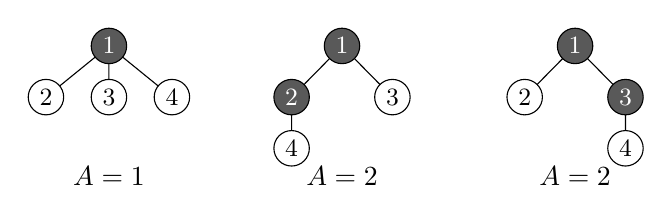
\begin{tikzpicture}[x=0.8cm,y=0.65cm,
 vertex/.style={circle,draw,minimum size=4.5mm,inner sep=0pt,font=\small},
 one/.style={vertex,fill=black!65,text=white},zero/.style={vertex,fill=white}]
 \begin{scope}
  \draw (0,2)--(-1,1) (0,2)--(0,1) (0,2)--(1,1);
  \node[one] at (0,2) {1};
  \node[zero] at (-1,1) {2}; \node[zero] at (0,1) {3};
  \node[zero] at (1,1) {4};
  \node at (0,-0.55) {$A=1$};
 \end{scope}
 \begin{scope}[shift={(3.7,0)}]
  \draw (0,2)--(-0.8,1)--(-0.8,0) (0,2)--(0.8,1);
  \node[one] at (0,2) {1}; \node[one] at (-0.8,1) {2};
  \node[zero] at (0.8,1) {3}; \node[zero] at (-0.8,0) {4};
  \node at (0,-0.55) {$A=2$};
 \end{scope}
 \begin{scope}[shift={(7.4,0)}]
  \draw (0,2)--(-0.8,1) (0,2)--(0.8,1)--(0.8,0);
  \node[one] at (0,2) {1}; \node[zero] at (-0.8,1) {2};
  \node[one] at (0.8,1) {3}; \node[zero] at (0.8,0) {4};
  \node at (0,-0.55) {$A=2$};
 \end{scope}
\end{tikzpicture}
\caption{Three four-vertex histories with the same root-state word
$(0,1,1,1)$ and different cumulative state-change counts $A$.
Labels give arrival order; filled vertices have final state one.
Replacing one history by another preserves every exterior state
history, providing the positive-variance argument.}
\label{fig:variancegadget}
\end{figure}

In $T_N$, $N>4$, condition on all vertex sets of size-four
fringes, their root-state words, and the contracted exterior history.
The interiors remain independent under this conditioning, each with
its weighted law conditional on the specified word. Changing one
interior while preserving its word leaves every exterior state
history unchanged: the actual birth labels are fixed, and the
exterior sees only this fringe root. Thus $A_N$ is the sum of a
fixed exterior contribution and independent interior scores.
The conditional variance formula gives
\[
 \operatorname{Var}(A_N)\ge
 v_\beta\eta_\beta\,\E N_{N,4}.
\]
Use \eqref{eq:affinefringe} and
\eqref{eq:varianceapproximationrate} to obtain the explicit bound
\begin{equation}\label{eq:positivePAvariance}
 \sigma_\beta^2\ge
 \frac{2(1+2\beta)(1+\beta)^2}
 {(2+\beta)(3+2\beta)^2(4+3\beta)(5+4\beta)}>0.
\end{equation}
This completes the one-root CLT. The displayed lower bound is not
claimed to be sharp, and no closed form for $\sigma_\beta^2$ is
asserted. Equation~\eqref{eq:varianceapproximationrate} characterizes
it by convergent variances from the cited additive-functional theorem.

\paragraph{The seed-edge degree law.}
Use the independent component construction and exact cumulative
identity from Appendix~\ref{app:degree}:
\[
 S_N=1+S_{m_1}^{(1)}+S_{m_2}^{(2)}+q(T_{m_2}^{(2)}),
 \qquad m_1+m_2=N.
\]
Conditional on sizes, the two internal histories are independent.
The last term divided by $\sqrt N$ tends to zero in $L^2$,
uniformly over splits, by \eqref{eq:rootL2}.
For any deterministic sequence of splits, pass to a subsequence on
which $m_i/N\to x_i$. If $x_i>0$, the one-root CLT gives an
independent Gaussian contribution with variance $x_i\sigma_\beta^2$.
If $x_i=0$, the uniform bounds
$\operatorname{Var}(S_m)=O_\beta(m)$ and
$\E S_m-\mu_\beta m=O_\beta(1)$ make that contribution vanish
in $L^2$. Since $x_1+x_2=1$, every such subsequence has the same
normal limit. This also proves convergence uniformly over splits,
so averaging over the random allocation preserves the limit.
The conditional variance of the sum of the two component costs is
$\sigma_\beta^2N+o(N)$ uniformly over splits; their conditional
mean differs from $\mu_\beta N$ by a bounded quantity.
The root correction is $o(\sqrt N)$ in $L^2$, so total variance
also converges as asserted in \eqref{eq:fullPAclt}.

Finally, \eqref{eq:fullPAclt} and the bounded mean correction imply
bounded second moments of $(S_N-\mu_\beta N)/\sqrt N$.
Its absolute values are uniformly integrable. Convergence to the
absolute first moment of the normal law proves
\eqref{eq:CLTabsmean} in both attachment conventions.
\end{proof}


\section{The maximum update}\label{sec:maximum}

The factorial tail bound immediately yields
$\PP(W_N\ge u)\le Nh_\beta H_\beta^{u-2}/(u-2)!$.
The main issue is obtaining a matching lower bound despite dependence
between successive insertions. A fringe whose last internal insertion
changes its root and $k$ old states certifies $W_N\ge k$ in the
global history. Its weighted EGF is
\[
 E_k(z)=\int_0^z\frac{H(t)^k}{k!}\,dt.
\]
The nonnegative coefficients of $H$ define an auxiliary sum of $k$
independent positive integer variables. This identifies a fringe size
of order $k$ at which the witness probability is at least
$c_\beta k^{-\zeta}H_\beta^k/k!$.
Lemma~\ref{lem:fringefacts} then gives a witness-count variance of
the same order as its mean. Stirling's formula locates both bounds
within a constant of the solution of
$r\log(r/(eH_\beta))=\log N$. Summable failure probabilities along
$N=2^j$ and monotonicity give the almost-sure bounded window.
Appendix~\ref{app:refinedmaximum} contains the full proof.

\section{Exact checks and scope}

The implementation and finite verification scripts are available in
the public repository\footnote{\url{https://github.com/mgalazka84/recursive-tree-exact-matching}.}
and in the source archive. Exact weighted enumeration covers all
5,914 increasing trees of sizes 1--8 and all 46,233 possible next
insertions, for seven reinforcement parameters and four degree
offsets. It checks sensitivity coefficients, update tails, fringe and
witness counts, cumulative means, and the seed-edge comparison.
The CLT checker verifies 252 centered variance identities across
all cutoffs and 3,474 local replacements, preserving every exterior
state at every arrival prefix. These checks support finite identities;
the asymptotic assertions rest on the proofs above and in the appendices.

Edge weights and deletions are outside the model. Our estimate for
the root's history uses fixed positive reinforcement. A CLT at the
uniform boundary, a closed-form variance evaluation, and a sharper
distributional description of the maximum remain questions for
further work.

\clearpage
\begin{thebibliography}{9}

\bibitem{AcarEtAl2004}
Acar, U.A., Blelloch, G.E., Harper, R., Vittes, J.L., Woo, S.L.M.:
Dynamizing static algorithms, with applications to dynamic trees and
history independence. In: Proceedings of the Fifteenth Annual ACM--SIAM
Symposium on Discrete Algorithms, pp. 524--533. SIAM (2004).
\url{https://www.cs.cmu.edu/~guyb/papers/ABHVW04.pdf}

\bibitem{GuptaSharma2009}
Gupta, M., Sharma, A.:
An $O(\log(n))$ fully dynamic algorithm for maximum matching in a tree.
arXiv:0901.2900 (2009). \url{https://arxiv.org/abs/0901.2900}

\bibitem{Janson2020}
Janson, S.:
On the independence number of some random trees.
Electronic Communications in Probability \textbf{25}, paper 63,
1--14 (2020). \doi{10.1214/20-ECP345}

\bibitem{PanholzerProdinger2007}
Panholzer, A., Prodinger, H.:
Level of nodes in increasing trees revisited.
Random Structures \& Algorithms \textbf{31}(2), 203--226 (2007).
\doi{10.1002/rsa.20161}

\bibitem{RalaivaosaonaWagner2019}
Ralaivaosaona, D., Wagner, S.:
A central limit theorem for additive functionals of increasing trees.
Combinatorics, Probability and Computing \textbf{28}(4), 618--637 (2019).
\doi{10.1017/S0963548318000585}

\bibitem{RudasTothValko2007}
Rudas, A., T\'oth, B., Valk\'o, B.:
Random trees and general branching processes.
Random Structures \& Algorithms \textbf{31}(2), 186--202 (2007).
\doi{10.1002/rsa.20137}

\bibitem{SeelbachWagner2022}
Seelbach Benkner, L., Wagner, S.:
Distinct fringe subtrees in random trees.
Algorithmica \textbf{84}, 3686--3728 (2022).
\doi{10.1007/s00453-022-01013-y}

\bibitem{TirodkarVishwanathan2019}
Tirodkar, S., Vishwanathan, S.:
Maximum matching on trees in the online preemptive and the incremental
graph models. Algorithmica \textbf{81}, 4275--4292 (2019).
\doi{10.1007/s00453-019-00593-6}

\end{thebibliography}

\clearpage
\appendix
\section{Preferential-attachment sensitivity and tails}\label{app:affinetails}

\begin{proof}[Proof of Theorem~\ref{thm:affine}]
Let $B_\beta(T)$ be the sum of weights
$1+\beta\lvert\ch(w)\rvert$ over insertion sites $w$ that change the
root state. We prove
\begin{equation}\label{eq:affinesensitivity}
 \E B_\beta(T_k)\le1\qquad(k\ge1).
\end{equation}
Give an increasing tree weight
$w_\beta(T)=\prod_v\prod_{j=0}^{|\ch(v)|-1}(1+\beta j)$.
Every history of size $k$ has the same denominator
$\tau_k=\prod_{i=1}^{k-1}Z_i$, so this is its probability multiplied
by $\tau_k$. The tree EGF $\mathcal T$ satisfies
\[
 \mathcal T'=\phi(\mathcal T),\qquad
 \phi(x)=(1-\beta x)^{-1/\beta},
\]
Let $A_i$ restrict this EGF to
root state $i$, and let $C$ additionally weight each tree by
$B_\beta(T)$. Then
\begin{equation}\label{eq:affineodes}
 A_0'=\phi(A_1),\qquad A_0+A_1=\mathcal T,\qquad
 C'=\phi'(A_1)(1+C),
\end{equation}
all series having zero constant term. The last identity follows from
\eqref{eq:Brec} with direct-root contribution
$1+\beta|\ch(r)|$: its EGF is
$\phi(A_1)+\beta A_1\phi'(A_1)=\phi'(A_1)$, and a sensitive child
contributes $\phi'(A_1)C$.

Write $\preceq$ for coefficientwise comparison. Differentiating gives
$C''=Q C'$ and $\mathcal T''=(Q+D)\mathcal T'$, where
\begin{align*}
 Q&=\frac{(1+\beta)\phi(\mathcal T)-\beta\phi(A_1)}{1-\beta A_1},\\
 D&=\frac{\beta}{1-\beta A_1}
       \bigl(A_0\phi'(\mathcal T)-\phi(\mathcal T)+\phi(A_1)\bigr).
\end{align*}
Both have nonnegative coefficients. For $Q$ use
$\phi(\mathcal T)+\beta(\phi(\mathcal T)-\phi(A_1))$ in the numerator.
For $D$, substituting a monomial $x^j$ into the parenthesis gives
$\sum_{\ell=2}^j(\ell-1)\binom j\ell A_0^\ell A_1^{j-\ell}$.
Since $C'(0)=\mathcal T'(0)=1$, coefficient induction yields
$C'\preceq\mathcal T'$ and hence $C\preceq\mathcal T$.
Now $[z^k]C/([z^k]\mathcal T)=\E B_\beta(T_k)$, proving
\eqref{eq:affinesensitivity}. 

A fringe subtree of size $k$ has total weight $Z_k$, independently
of its shape. Conditional on receiving an insertion, its parent is
chosen according to the same affine rule. Thus, conditional on size,
its increasing relabeling has law $T_k$. For each vertex the expected
weighted sensitivity is at most one. Averaging over parent choices,
\[
 \E K_n=\frac1{Z_n}\E\sum_{v\in T_n}B_\beta((T_n)_v)
 \le\frac n{Z_n}.
\]
Pathwise, $U_n=1+$ the number of changed nonroot vertices. The same
argument omitting the root gives its sharper bound in
\eqref{eq:affinemeans}. Lemma~\ref{lem:implementation} proves the
recourse, time, space, and query assertions. The tail proof follows below.
\end{proof}

We prove the remaining claims of Theorem~\ref{thm:affine}. Fix $\beta>0$
and put $\zeta=(1+\beta)^{-1}$ and $q=1-\zeta$. All generating
functions in this appendix use the weights $w_\beta$ from its proof.
For $s>0$, let $B_{\beta,s}(T)$ weight a sensitive insertion site $w$
by $(1+\beta|\ch(w)|)s^{\operatorname{depth}(w)}$, and let $C(z,s)$
be its weighted EGF. The marked recurrence is \eqref{eq:affinemarked}.
For $\beta>0$,
\[
 \mathcal T(z)=\frac{1-(1-z/\zeta)^{\beta/(1+\beta)}}\beta,
 \qquad \mathcal T(\zeta)=1/\beta.
\]
Since $A_0(z)\succeq z$, we have
$1-\beta A_1(\zeta)=\beta A_0(\zeta)\ge\beta\zeta>0$.
Consequently both
\[
 h_\beta:=\phi'(A_1(\zeta))<\infty,
 \qquad H_\beta:=H(\zeta)<\infty
\]
are finite and positive, and
$\partial_z C(\zeta,s)=h_\beta e^{sH_\beta}$.
All coefficients of $C(z,s)$ in both variables are nonnegative.

Use Lemma~\ref{lem:fringefacts} for fringe counts and their conditional laws.

Put $b_k(s)=[z^k]C(z,s)$. A changed chain contributes once at each
of its ancestors, hence
$F_{n,\beta}(s):=\E\sum_{j=1}^{K_n}s^{j-1}$ equals
$Z_n^{-1}\E\sum_v B_{\beta,s}((T_n)_v)$.
Using \eqref{eq:affinefringe} and
\[
 [z^k]\mathcal T
 =\frac{\zeta^{1-k}\Gamma(k-1+\zeta)}{\Gamma(\zeta)k!}
\]
gives the exact formula
\begin{equation}\label{eq:affineF}
 F_{n,\beta}(s)=
 \sum_{k=1}^{n-1}
 \frac{\zeta\Gamma(\zeta)k!}{\Gamma(k+1+\zeta)}
       b_k(s)\zeta^k
 +\frac{\Gamma(\zeta)n!}{\Gamma(n+\zeta)}b_n(s)\zeta^n.
\end{equation}
The first coefficient decreases with $k$, starting at
$1/(1+\zeta)$. The final coefficient divided by $n$ decreases with
$n$, starting at $1/\zeta$. Thus every coefficient multiplying
$b_k(s)\zeta^k$ in \eqref{eq:affineF} is at most $k/\zeta$, and
\[
 F_{n,\beta}(s)\le\sum_{k\ge1} k b_k(s)\zeta^{k-1}
 =h_\beta e^{sH_\beta}.
\]


The inequality also holds coefficientwise in $s$. Extracting the
coefficient of $s^{k-1}$ proves \eqref{eq:factorialupper}.
For $s\ge1$ the geometric-sum identity gives
\begin{equation}\label{eq:affinepgfbound}
 \E s^{K_n}\le1+(s-1)h_\beta e^{sH_\beta}.
\end{equation}
In particular $\PP(K_n\ge k)\le\exp\{-k\log k+O_\beta(k)\}$
uniformly in $n$. No independence of successive costs is used.
\section{The preferential limiting law}\label{app:affinelimit}

\begin{proof}[Proof of Theorem~\ref{thm:affinelimit}]
Fix $\beta>0$ and $s>0$, and retain the notation of
Appendix~\ref{app:affinetails}. The series
$\sum_{j\ge1}j b_j(s)\zeta^{j-1}=\partial_z C(\zeta,s)$ converges.
The last term in \eqref{eq:affineF} is at most
$n b_n(s)\zeta^{n-1}$, and therefore tends to zero. The other terms
are nonnegative. The beta-integral identity
\[
 d_j:=\frac{\zeta\Gamma(\zeta)j!}{\Gamma(j+1+\zeta)}
   =\zeta\int_0^1x^j(1-x)^{\zeta-1}\,dx
\]
and termwise integration yield
\[
 F_{n,\beta}(s)\longrightarrow
 \sum_{j\ge1}d_j b_j(s)\zeta^j
 =\zeta\int_0^1(1-x)^{\zeta-1}C(\zeta x,s)\,dx
 =\Phi_\beta(s).
\]
Since $H(\zeta)<\infty$, this integral is continuous at $s=1$.
The geometric-sum identity and the continuity theorem for probability
generating functions prove convergence to \eqref{eq:affinelimitpgf}.
Uniform exponential-moment bounds \eqref{eq:affinepgfbound} imply
uniform integrability of every fixed polynomial moment. The root
changes with probability at most $1/Z_n$, by
\eqref{eq:affinesensitivity}; hence $U_n=K_n+1-R_n$ gives the
assertions for $U_n$. At $s=0$, point-probability convergence and
continuity give the same formula.

Expanding $(e^{sH}-1)/s$ in nonnegative powers of $s$ and comparing
coefficients in
$\Phi_\beta(s)=\sum_{k\ge1}\PP(K_\beta\ge k)s^{k-1}$ proves
\eqref{eq:affinelimittails}. Finally, convergence of the means and
\eqref{eq:affinemeans} give $\Phi_\beta(1)\le\zeta$.
\end{proof}

\paragraph{Sharp limiting tails.}
Write $H_\beta=H(\zeta)$ and $h_\beta=H'(\zeta)$, both finite and
positive. We prove \eqref{eq:affinelimitsharp}.
Indeed, $H(\zeta x)=H_\beta-\zeta h_\beta(1-x)+o(1-x)$.
In \eqref{eq:affinelimittails}, put $y=1-x$ and scale $y$ by $1/k$.
For small $y$, the ratio $H(\zeta(1-y))/H_\beta$ is at most
$\exp(-cy)$ for some $c>0$; on a fixed interval away from zero it
is bounded strictly below one. Dominated convergence on the scaled
integral therefore gives
$\Gamma(\zeta)(H_\beta/(\zeta h_\beta k))^\zeta$ after extracting
$H_\beta^k$. Multiplication by $\zeta/k!$ proves
\eqref{eq:affinelimitsharp}. This assertion is for fixed $\beta>0$.

\paragraph{Certified approximation.}
Formula \eqref{eq:affineF} also yields rational interval bounds when
$\beta$ is rational. For either $D(z)=C(z,1)$ or
$D(z)=H(z)^k/k!$, write $d_j$ as above and truncate
$\sum_{j\ge1}d_j\zeta^j[z^j]D$ at $j=L$. This gives a lower bound
for $\E K_\beta$ or $\PP(K_\beta\ge k)$, respectively. Since
$0\preceq H^k/k!\preceq C(z,1)\preceq\mathcal T(z)$,
its remainder is at most
\begin{equation}\label{eq:affinecertified}
 \sum_{j>L}d_j\zeta^j[z^j]\mathcal T
 =\sum_{j>L}\frac{\zeta^2}{(j-1+\zeta)(j+\zeta)}
 =\frac{\zeta^2}{L+\zeta}.
\end{equation}
The checker implements these bounds in exact rational arithmetic.


\section{A bounded window for the preferential maximum}\label{app:refinedmaximum}

\begin{proof}[Proof of Theorem~\ref{thm:affinerefinedmax}]
Fix $\beta>0$ and abbreviate $H=H_\beta$, $h=h_\beta$,
$\zeta=(1+\beta)^{-1}$ and $r=r_\beta(N)$. The upper bound follows
from \eqref{eq:factorialupper} and $U_n\le K_n+1$: for integers
$u\ge2$,
\begin{equation}\label{eq:maximumfactorialupper}
 \PP(W_N\ge u)\le Nh\frac{H^{u-2}}{(u-2)!}.
\end{equation}
We next construct lower-bound witnesses on the same factorial scale.

For an increasing tree of size $j+1$, call its last insertion a
$k$-witness if it changes the root and exactly $k$ old states.
Deleting its largest-labelled leaf leaves a root-sensitive insertion
site at depth $k-1$ in a size-$j$ tree. Its weight is the old tree
weight times the insertion weight. By \eqref{eq:affinemarked},
the weighted EGF of these new trees is
\begin{equation}\label{eq:witnessEGF}
 E_k(z)=\int_0^z\frac{H(t)^k}{k!}\,dt.
\end{equation}
Indeed, $[s^{k-1}]C(z,s)=H(z)^k/k!$, and integration changes
the denominator $j!$ into $(j+1)!$ when the largest label is inserted.

Introduce a positive integer-valued variable $Y$ by
\[
 \PP(Y=j)=\frac{[z^j]H(z)\,\zeta^j}{H},\qquad
 a:=\E Y=\frac{\zeta h}{H}<\infty.
\]
In particular $a\ge1$. Let $V_k=Y_1+\cdots+Y_k$ for independent
copies. Markov's inequality gives
$\PP(k\le V_k\le\lceil2ak\rceil)\ge1/2$.
There is therefore an integer $j=j(k)$ in this interval such that
$\PP(V_k=j)\ge c_1/k$, where constants depend only on $\beta$.
Write $t_m=[z^m]\mathcal T(z)$. For this $j$, the probability
$p_{j+1,k}$ that a size-$(j+1)$ tree is a $k$-witness is exactly
\begin{align}
 p_{j+1,k}
 &=\frac{[z^j]H(z)^k}{k!(j+1)t_{j+1}}\notag\\
 &=\frac{\Gamma(\zeta)j!}{\Gamma(j+\zeta)}
      \frac{H^k}{k!}\,\PP(V_k=j)
 \ge c_2\,k^{-\zeta}\frac{H^k}{k!}.
 \label{eq:witnessprobability}
\end{align}
Here $j!/\Gamma(j+\zeta)\asymp j^{1-\zeta}$ and $j\asymp k$.

Let $X_{N,k}$ count such size-$(j+1)$ fringe witnesses in $T_N$.
For $j+1<N$, \eqref{eq:affinefringe} gives
\begin{equation}\label{eq:witnessmean}
 \lambda_{N,k}:=\E X_{N,k}
 \ge c_3\,\frac{N H^k}{k!\,k^{2+\zeta}}.
\end{equation}
Lemma~\ref{lem:fringefacts}
applies also to events retaining the relative order of labels.
Consequently, conditional on the number of size-$(j+1)$ fringes,
$X_{N,k}$ is binomial with success probability $p_{j+1,k}$.
The size-uniform variance bound then yields
$\operatorname{Var}X_{N,k}=O_\beta(\lambda_{N,k})$.
Every witness certifies $W_N\ge k$: at its last internal birth,
all its then existing descendants belong to this final fringe,
and the $k$ local state changes are also changes in the full tree.
External insertions do not affect the subtree states. Hence
\begin{equation}\label{eq:witnessfailure}
 \PP(W_N<k)\le\PP(X_{N,k}=0)
 \le C_\beta\,\lambda_{N,k}^{-1}.
\end{equation}

To locate the window, let $f(x)=x\log(x/(eH))$; then
$f(r)=\log N$. Stirling's formula, uniformly for bounded real $b$
with $r+b$ an integer, gives
\begin{equation}\label{eq:windowstirling}
 N\frac{H^{r+b}}{(r+b)!}
 =\Theta_\beta(r^{-b-1/2}).
\end{equation}
For any fixed $D>7/2+\zeta$, put
$u_N=\lceil r+D\rceil$ and $k_N=\lfloor r-D\rfloor$.
Equations \eqref{eq:maximumfactorialupper}--\eqref{eq:windowstirling}
give
\[
 \PP(W_N\ge u_N)=O_\beta(r^{3/2-D}),\qquad
 \PP(W_N<k_N)=O_\beta(r^{5/2+\zeta-D}).
\]
For instance $D=6$ makes both bounds summable along $N=2^i$,
because $r_\beta(2^i)\asymp i/\log i$.
The first Borel--Cantelli lemma gives a bounded window almost surely
along this subsequence. Also
$r_\beta(2N)-r_\beta(N)=O_\beta(1/\log r_\beta(N))=o(1)$,
by $f'(x)=\log(x/H)$.
Monotonicity of $W_N$ and $r_\beta(N)$ therefore interpolates the
bounded window to every sufficiently large $N$.

For the seed-edge model, use $W_N^F\le W_N\le W_N^F+1$ from
Appendix~\ref{app:degree}. Both infinite component histories
satisfy the bounded window on a common probability-one event.
The larger component has at least $N/2$ vertices and
$r_\beta(N)-r_\beta(N/2)=o(1)$, while both component maxima are
bounded above by their size-$N$ maxima. This proves the same result.

Finally, solving $r\log(r/(eH))=L$ gives
\[
 r=\frac L\ell+
   \frac{L(\log\ell+1+\log H)}{\ell^2}
   +O_\beta\!\left(\frac{L(\log\ell)^2}{\ell^3}\right).
\]
This follows by substitution in $f(r)=L$ and the mean value theorem,
or by the expansion of the positive Lambert-$W$ branch.
The bounded random error is absorbed in this remainder, proving
\eqref{eq:secondordermaximum}.
\end{proof}

\section{The cumulative mean and finite root history}\label{app:affinetotal}

\begin{proof}[Proof of Theorem~\ref{thm:affinetotal}]
Fix $\beta>0$ and write $C(z)=C(z,1)=e^{H(z)}-1$,
$\zeta=(1+\beta)^{-1}$, and
\[
 a_j=[z^j]C(z)\,\zeta^j,\qquad
 d_j=\frac{\zeta\Gamma(\zeta)j!}{\Gamma(j+1+\zeta)},\qquad
 b_j=d_j a_j.
\]
Then $\kappa_\beta:=\sum_{j\ge1}b_j=\Phi_\beta(1)$ and
$\mu_\beta=1+\kappa_\beta$.
The final term of \eqref{eq:affineF} at $s=1$ is exactly the root
flip probability
\[
 p_n:=\PP(R_n=1)
 =\frac{\Gamma(\zeta)n!}{\Gamma(n+\zeta)}a_n.
\]
It cancels when $\E U_n=1+\E K_n-p_n$ is formed. Thus
\begin{equation}\label{eq:exactPAtotalmean}
 \E U_n=1+\sum_{j<n}b_j,\qquad
 \E S_N=N-1+\sum_{j=1}^{N-2}(N-1-j)b_j.
\end{equation}
All series are nonnegative and
$\sum j a_j=\zeta C'(\zeta)<\infty$;
also $0<d_j\le1$. Hence $\sum j b_j<\infty$. Set
\begin{equation}\label{eq:meancorrection}
 \begin{split}
 c_\beta&=\mu_\beta+\sum_{j\ge1}j b_j\\
 &=\mu_\beta+\zeta^2\int_0^1
 x(1-x)^{\zeta-1}H'(\zeta x)e^{H(\zeta x)}\,dx.
 \end{split}
\end{equation}
The exact remainder in
$\E S_N-(\mu_\beta N-c_\beta)$ is
$\sum_{j\ge N-1}(j-N+1)b_j$, which is nonnegative and tends to
zero. This proves the mean assertion with its explicit correction.

Let $q(T)$ again count changes of the root during its increasing-label
history. Since $\Gamma(\zeta)n!/\Gamma(n+\zeta)\le n/\zeta$,
\begin{equation}\label{eq:PArootfinite}
 \sup_n\E q(T_n)=\sum_{n\ge1}p_n
 =:Q_\beta\le C'(\zeta)=h_\beta e^{H_\beta}<\infty.
\end{equation}
Along the growth coupling, $q(T_n)$ increases to an integrable,
almost surely finite $q_\infty$. In particular the root state changes
only finitely often almost surely. Moreover
$\E q(T_k)^2\le(k-1)Q_\beta$.


This proves Theorem~\ref{thm:affinetotal}. The seed-edge mean and
the cumulative comparison used in the CLT are recorded in
Appendix~\ref{app:degree}.
\end{proof}
\section{Transfer to degree-based attachment}\label{app:degree}
We prove Corollary~\ref{cor:degree} and the comparisons used above.
For the mean bound, every nonroot fringe uses weights
$(1+\delta)+|\ch(v)|$, and its unnormalized expected root
sensitivity is at most $1+\delta$ by \eqref{eq:affinesensitivity}.
The total attachment weight is $(2+\delta)n-2$. Since $U_n$ is one
plus the number of changed nonroot vertices, summing these sensitivities
proves \eqref{eq:degreemean}. Lemma~\ref{lem:implementation} and
$K_n\le U_n$ give constant expected time and recourse.

\paragraph{Independent components.}
Delete the seed edge $\{a,b\}$ and regard the two components as
rooted at $a,b$. Every vertex, including each component root, has
one incident edge outside its set of children in this forest. Thus
its attachment weight is
$(1+\delta)+|\ch(v)|$, and division by $1+\delta$ gives
\eqref{eq:affineparent} with $\beta=1/(1+\delta)$.
A component of size $m$ has normalized weight $Z_m$.

Construct two independent infinite affine growth histories and an
independent allocation process. At component sizes $(m_1,m_2)$,
choose component $i$ with probability $Z_{m_i}/(Z_{m_1}+Z_{m_2})$
and reveal its next insertion. This generates exactly the seed-edge
law. In particular, conditional on component sizes, their internal
histories have the corresponding independent affine laws. At global
size $n$, the total normalized weight is
$Z_{m_1}+Z_{m_2}=(1+\beta)n-2\beta$.

Let $K_n^F,U_n^F$ be the update counts when propagation stops at the
root of the selected component. The probability of selecting a
component of size less than any fixed $L$ is at most
$2Z_L/((1+\beta)n-2\beta)$, which tends to zero. Conditioning on
component sizes and applying Theorem~\ref{thm:affinelimit} therefore
shows $K_n^F\xrightarrow{d}K_\beta$ and
$U_n^F\xrightarrow{d}K_\beta+1$.

Root the full tree at $a$. For an insertion in its component,
$U_n=U_n^F$; for one in the component at $b$,
$U_n=U_n^F+R_n^F$, where $R_n^F$ indicates a change at $b$.
In either case $|K_n-K_n^F|\le1$, and a difference in either count
requires the selected component root to change. By
\eqref{eq:affinesensitivity}, that event has probability at most
$2/((1+\beta)n-2\beta)$. Hence the full-tree counts have the same
limits. Moreover $K_n\le K_n^F+1$, so uniform exponential-moment
bounds persist. Uniform integrability, using a larger fixed
exponential moment when necessary, proves convergence of the
polynomial moments and the PGFs for every fixed $s>0$.


\paragraph{Cumulative and maximum comparisons.}
Let $S_m^{(i)},W_m^{(i)}$ be the within-component cumulative cost
and maximum, with $S_1^{(i)}=W_1^{(i)}=0$.
At global size $N$, $m_1+m_2=N$, and the pointwise inspection
comparison above gives
\begin{equation}\label{eq:degreecumulative}
 S_N=1+S_{m_1}^{(1)}+S_{m_2}^{(2)}+q(T_{m_2}^{(2)}).
\end{equation}
The initial one creates the seed edge. The one-root mean expansion
holds with a uniformly bounded remainder over all positive sizes;
also $\E q(T_m)\le Q_\beta$. Conditioning on sizes therefore gives
$\E S_N=\mu_\beta N+O_\beta(1)$.
With $W_N^F=\max\{W_{m_1}^{(1)},W_{m_2}^{(2)}\}$,
\begin{equation}\label{eq:degreemaximum}
 W_N^F\le W_N\le W_N^F+1.
\end{equation}
At least one component has size at least $N/2$. On the common
probability-one event of the two one-root maximum laws,
$r_\beta(N)-r_\beta(N/2)=o(1)$ and monotonicity transfer the
bounded window to the full tree. The transfer of the CLT, variance
asymptotic, and absolute mean error was proved in
Section~\ref{sec:clt} using \eqref{eq:degreecumulative}.

\end{document}
